\documentclass[11pt,a4paper]{article}
\usepackage{tikz}
\usepackage{mathpazo}
\usepackage{amssymb}
\usetikzlibrary{mindmap,trees}
\usetikzlibrary{arrows,shapes, trees, backgrounds}

\begin{document}
The following code is taken from \textbf{PGF/TikZ- Graphics for \LaTeX}, Meik Hellmund, Uni Leipzig
\section*{Page 3}

part 1:

\begin{center}
\tikz \draw (0pt,0pt) -- (20pt,6pt);
\tikz \fill[orange] (0,0) circle (1ex);
\end{center}

part 2:

\begin{center}
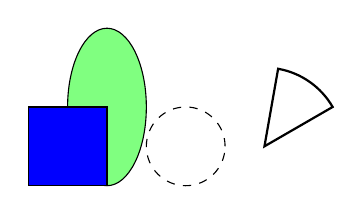
\begin{tikzpicture}
\draw[style=dashed] (2,.5) circle (0.5);
\draw[fill=green!50] (1,1) ellipse (.5 and 1);
\draw[fill=blue] (0,0) rectangle (1,1);
\draw[style=thick] (3,.5) -- +(30:1) arc(30:80:1) -- cycle;
\end{tikzpicture}
\end{center}

\section*{Page 4}

\begin{center}
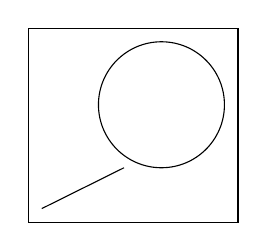
\begin{tikzpicture}[scale = .8, show background rectangle]
\draw (2,2) circle (1);
\draw (1 mm, 10 pt) -- (4em, 1);
\end{tikzpicture}
\end{center}

\section*{Page 5, Paths}

part 1:

\begin{center}
\tikz \path[draw] (1,1)--(2,2)--(3,1);\\
\tikz \path[draw, line width=4pt](1,1)--(2,2)--(3,1)--cycle;\\
\tikz \path[draw, fill=green!20] (1,1)--(2,2)--(3,1)--cycle;\\
\tikz \path[fill=green] (1,1)--(2,2)--(3,1)--cycle;
\end{center}

part 2:

\begin{center}
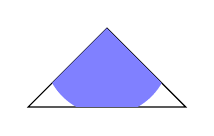
\begin{tikzpicture}
\path[clip,draw] (1,1)--(2,2)--(3,1)--cycle;
\path[fill=blue!50] (2,1.7) circle (.8);
\end{tikzpicture}
\end{center}

\section*{Page 6, Shading}
part 1:

\begin{center}
\tikz \path[shade, draw] (1,1)--(2,2)--(3,1)--cycle;\\
\tikz \shade[left color = red] (1,1)--(2,2)--(3,1)--cycle;\\
\tikz \shade[top color=red, bottom color=green] (0,0) rectangle (2,1);\\
\tikz \shade[draw, shading=radial, inner color=blue] (0,0) rectangle (2,1);\\
\tikz \shade[shading=ball, ball color=blue] (0,0) rectangle (2,1);
\end{center}

part 2:

\begin{center}

\begin{tikzpicture}
\shade[shading=ball,ball color=blue] (0,0) circle (.3);
\shade[shading=ball,ball color=white] (1,0) circle (.3);
\shade[shading=ball,ball color=black] (2,0) circle (.3);
\end{tikzpicture}
\end{center}

\section*{Page 7, Simple shapes}

part 1:
\begin{center}
\tikz \draw (0,0) rectangle (2,1);\\
\tikz \draw[color=red] (0,0) circle (.5);\\
\tikz \draw (0,0) ellipse (.7 and 0.5);
\end{center}

Polar coordinates:

\begin{center}
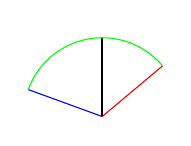
\begin{tikzpicture}
\draw[color=red] (0,0) -- (40:1);
\draw[color=blue] (0,0) -- (160:1);
\draw[thick] (0,0) -- (90:1);
\draw[color=green] (40:1) arc (40:160:1);
\end{tikzpicture}
\end{center}

\section*{Page 8, Curved lines}

part 1:

\begin{center}
\tikz \draw[line width=2pt] (0,0) .. controls(1,1) .. (3,0);
\end{center}

part 2:

\begin{center}
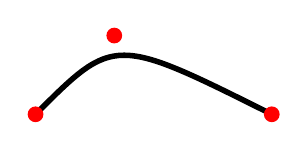
\begin{tikzpicture}
\draw[line width=2pt] (0,0) .. controls(1,1) .. (3,0);
\fill[fill=red] (0,0) circle (.1);
\fill[fill=red] (1,1) circle (.1);
\fill[fill=red] (3,0) circle (.1);
\end{tikzpicture}
\end{center}

part 3:

\begin{center}
\tikz \draw[line width=8pt] (0,0) .. controls(1,0) and (1,1) .. (0,1);
\end{center}

part 4:

\begin{center}

\begin{tikzpicture}
\draw[line width=8pt] (0,0) .. controls(1,0) and (1,1) .. (0,1);
\fill[fill=red] (0,0) circle (.1);
\fill[fill=red] (1,0) circle (.1);
\fill[fill=red] (1,1) circle (.1);
\fill[fill=red] (0,1) circle (.1);
\end{tikzpicture}
\end{center}

\section*{Page 9}

part 1:

\begin{center}
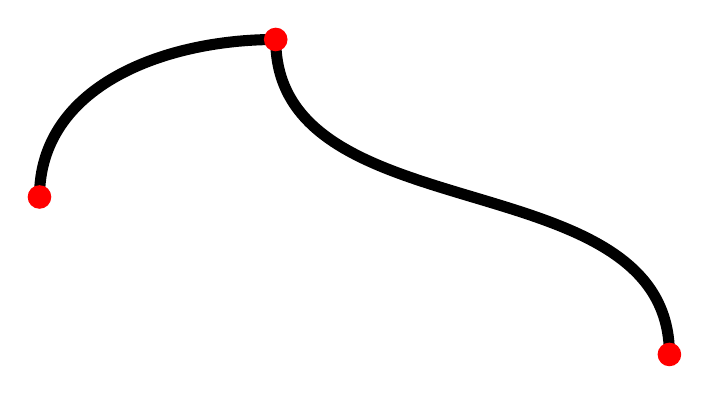
\begin{tikzpicture}
\draw[line width=4pt] (0,0) to [out=90, in=180] (3,2) to [out=-90, in=90] (8,-2);
\fill[fill=red] (0,0) circle (.15);
\fill[fill=red] (3,2) circle (.15);
\fill[fill=red] (8,-2) circle (.15);
\end{tikzpicture}
\end{center}

\section*{Page 10, Arrows, dash patterns}
\begin{center}
\tikz \draw[->] (0,0) -- (1,0);\\
\tikz \draw[dotted,>->>] (0,0) -- (1,0);\\
\tikz \draw[|<->|] (0,0) -- (1,0);\\
\tikz \draw[dashed,o-)] (0,0) -- (1,0);\\
\tikz \draw[loosely dashed] (0,0) -- (1,0);\\
\tikz \draw[densely dotted] (0,0) -- (1,0);\\
\tikz \draw[->] (0,0) .. controls (.2,-.2) .. (1,0);
\end{center}

\section*{Page 11, Clipping and scope}
\begin{center}
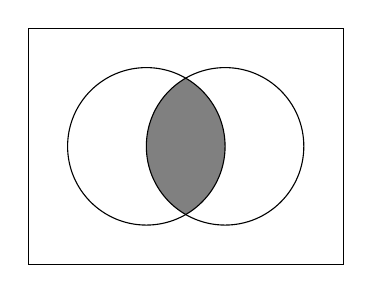
\begin{tikzpicture}
\draw (-2, 1.5) rectangle (2, -1.5);
\begin{scope}
\clip (-0.5,0) circle (1);
\clip (0.5,0) circle (1);
\fill[color=gray] (-2, 1.5) rectangle (2,-1.5);
\end{scope}
\draw (-0.5,0) circle (1);
\draw (0.5,0) circle (1);
\end{tikzpicture}
\end{center}

\section*{Page 12, Nodes}
part 1:

\begin{center}
\tikz \path[draw] (0,0) node {A} -- (1,0) -- (1,1) node {B};
\end{center}

part 2:

\begin{center}
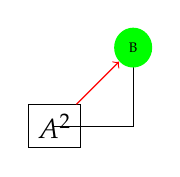
\begin{tikzpicture}
\draw (0,0) node[draw] (nodeA) {$A^2$} --(1,0)--(1,1) node[ellipse,fill=green] (nodeB) {\tiny B};
\draw[red,->] (nodeA) -- (nodeB);
\end{tikzpicture}
\end{center}

In the other suggested way:

\begin{center}
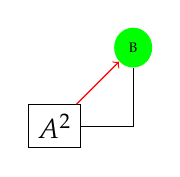
\begin{tikzpicture}
\node[draw] (nodeA) {$A^2$};
\node[ellipse,fill=green] (nodeB) at (1,1) {\tiny B};
\path[draw] (nodeA) -- (1,0) -- (nodeB);
\draw[red,->] (nodeA) -- (nodeB);
\end{tikzpicture}
\end{center}

\section*{Page 13}

\begin{center}
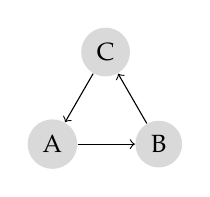
\begin{tikzpicture}[scale=.9, transform shape]
\tikzstyle{every node} = [circle, fill=gray!30]
\node (a) at (0,0) {A};
\node (b) at (0:1.5) {B};
\node (c) at (60:1.5) {C};
\foreach \from/\to in {a/b, b/c, c/a}
            \draw[->] (\from) -- (\to);
\end{tikzpicture}
\end{center}

\section*{Page 14}

part 1:

\begin{center}
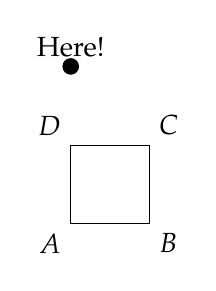
\begin{tikzpicture}
\fill (0,2) circle (3pt) node[above] {Here!};
\draw (0,0) node[below left] {$A$} --
      (1,0) node[below right] {$B$} --
      (1,1) node[above right] {$C$} --
      (0,1) node[above left] {$D$} -- cycle;
\end{tikzpicture}
\end{center}

part 2:

\begin{center}
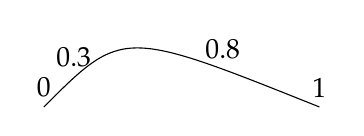
\begin{tikzpicture}
\draw (0,0) .. controls(1,1) .. (3.5,0)
      node[pos=0, above] {0}
      node[pos=0.3, left] {0.3}
      node[pos=0.8, above] {0.8}
      node[pos=1, above] {1};
\end{tikzpicture}
\end{center}

\section*{Page 15, Some more examples}
part 1:

\begin{center}
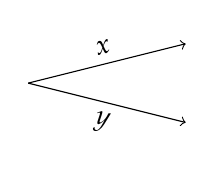
\begin{tikzpicture}
\draw[->] (0,0) -- (2,.5) node[pos=0.5, sloped, above] {$x$};
\draw[->] (0,0) -- (2,-.5) node [pos=0.5,sloped,below] {$y$};
\end{tikzpicture}
\end{center}

part 2:

\begin{center}
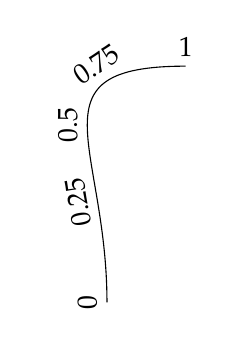
\begin{tikzpicture}
\tikzstyle{every node} = [sloped, above, allow upside down]
\draw (0,0) .. controls (up:2cm) and +(left:2cm).. (1,3)
\foreach \p in {0,0.25,...,1} {node[pos=\p]{\p}};
\end{tikzpicture}
\end{center}

\section*{Page 16}
\begin{center}
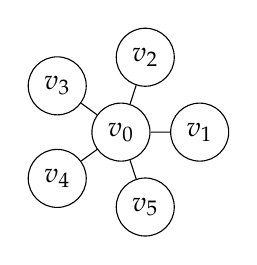
\begin{tikzpicture}
\tikzstyle{every node} = [draw, shape=circle];
\node (v0) at (0:0) {$v_0$};
\node (v1) at (0:1) {$v_1$};
\node (v2) at (72:1) {$v_2$};
\node (v3) at (2*72:1) {$v_3$};
\node (v4) at (3*72:1) {$v_4$};
\node (v5) at (4*72:1) {$v_5$};
\draw (v0) -- (v1)
      (v0) -- (v2)
      (v0) -- (v3)
      (v0) -- (v4)
      (v0) -- (v5);
\end{tikzpicture}
\end{center}

\section*{Page 17}
\usetikzlibrary{calc,through}

\begin{center}
\begin{tikzpicture}[scale=1.2]
\coordinate[label=left:$A$] (A);
\coordinate[label=right:$B$] (B) at (1.25,0.25);
\draw (A) -- (B);
\node (D) [draw,circle through=(B),label=left:$D$] at (A) {};
\node (E) [draw,circle through=(A),label=right:$E$] at (B) {};
\coordinate[label=above:$C$] (C) at (intersection 2 of D and E);
\draw[red] (A) -- (C);
\draw[red] (B) -- (C);
\end{tikzpicture}
\end{center}

\section*{Page 18, Loops}
\begin{center}
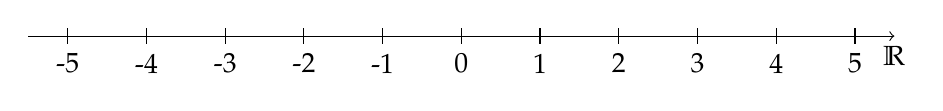
\begin{tikzpicture}
\draw[->] (-5.5,0) -- (5.5,0) node [below] {$\mathbb{R}$};
\foreach \x in {-5,...,5}
\draw (\x,0.1) -- (\x,-0.1) node[below] {\x};
\end{tikzpicture}
\end{center}

\begin{center}

\begin{tikzpicture}
\foreach \x in{1,3,...,10}
\shade[ball color=red!\x 0!green] (\x,0) circle (3mm);
\end{tikzpicture}
\end{center}

\begin{center}
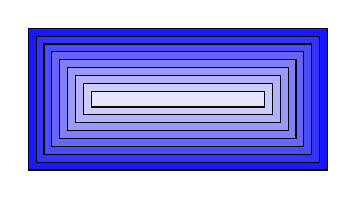
\begin{tikzpicture}
\foreach \x in {9,...,1}
\draw[fill=blue!\x0] (-0.1*\x -1, 0.1*\x) rectangle (0.1*\x + 1, -0.1*\x);
\end{tikzpicture}
\end{center}

\section*{Page 19, Referencing nodes outside the current picture}
\tikzstyle{every picture} += [remember picture]
\begin{itemize}
\renewcommand{\labelitemi}{$\blacktriangleright$}
\item Add the overlay to all \tikz[baseline,inner sep=0] \node[anchor=base] (n1) {paths}; that reference nodes outside the current picture
\item Run pdflatex twice!
\item The word "\tikz[baseline, inner sep=0] \node[anchor=base] (n2) {paths};" above and here is really a node: ...
\end{itemize}

\begin{center}
\tikz[overlay]\draw[thick,green,->] (n2) -- (n1);
\end{center}

\section*{Page 20, Integration with Beamer}
\[y = \tikz[baseline]{\node[fill=blue!50,anchor=base](t1) {$a$};}x +
      \tikz[baseline]\node[fill=red!50,anchor=base](t2){$b$};\]
\begin{itemize}
\item[]\tikz \node[fill=blue!50,draw,circle] (n1) {}; slope
\item[] \tikz\node[fill=red!50,draw,circle] (n2) {}; y-intercept
\end{itemize}

\begin{center}
\begin{tikzpicture}[overlay]
\path[blue,->] (n1.north) edge [out=60, in=135] (t1.north west);
\path[red,->] (n2.south) edge [out=-70, in=-110] (t2.south);
\end{tikzpicture}
\end{center}

\section*{Page 21, Some Libraries}
\begin{center}
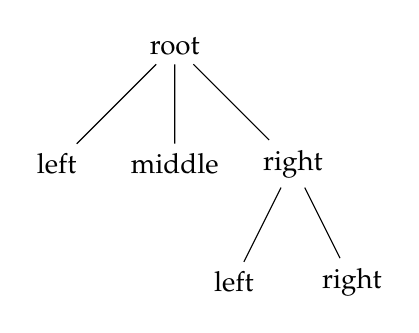
\begin{tikzpicture}
\tikzstyle{every node} = [align=center]
\node(root) {root}
child {node {left}}
child {node {middle}}
child {node {right}
child {node {left}}
child {node {right}}};
\end{tikzpicture}
\end{center}

\begin{center}
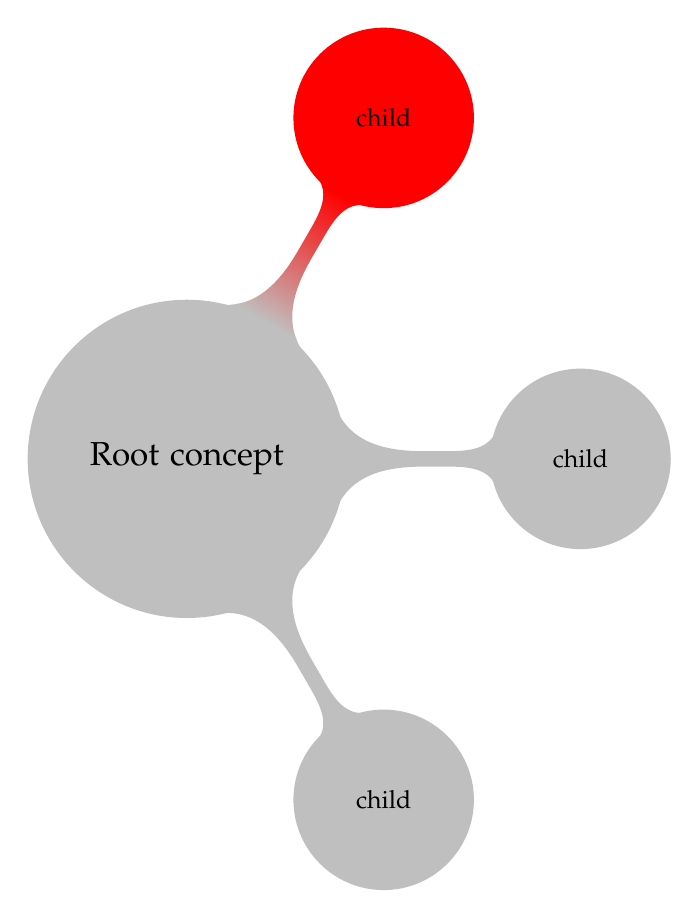
\begin{tikzpicture}
\path[mindmap,concept color=gray!50]
node[concept] {Root concept}
[clockwise from=60]
child[concept color=red] {
   node[concept] {child}}
child {
  node[concept] {child}}
child { node[concept] {child} };
\end{tikzpicture}
\end{center}
\end{document}
